%----------------------------------------------------------------------------------------
%	PACKAGES AND OTHER DOCUMENT CONFIGURATIONS
%----------------------------------------------------------------------------------------

\documentclass[12pt, a4paper, oneside]{article} % Paper size, default font size and one-sided paper

\usepackage{nomencl}
\usepackage{hyperref}
\usepackage{enumitem}
\usepackage{setspace}
\usepackage{fancyhdr}
\usepackage[utf8]{inputenc}
\usepackage{graphicx}
\usepackage{color}
\usepackage{epstopdf}
\usepackage[final]{pdfpages}
\usepackage[utf8]{inputenc}
\usepackage{float}

\usepackage[margin=1in]{geometry}
\usepackage[square, numbers, comma, sort&compress]{natbib} 
%\makenomenclature
\renewcommand{\nomname}{Time Zones}
\newcommand{\solidareit}{\textsc{s}olidare-\textsc{it} }
\title{\ttitle} % Defines the thesis title - don't touch this

\usepackage{listings}
\usepackage{color}

\definecolor{dkgreen}{rgb}{0,0.6,0}
\definecolor{gray}{rgb}{0.5,0.5,0.5}
\definecolor{mauve}{rgb}{0.58,0,0.82}

\setitemize{noitemsep}

\lstset{frame=tb,
  aboveskip=3mm,
  belowskip=3mm,
  showstringspaces=false,
  columns=flexible,
  basicstyle={\small\ttfamily},
  numbers=none,
  numberstyle=\tiny\color{gray},
  keywordstyle=\color{blue},
  commentstyle=\color{dkgreen},
  stringstyle=\color{mauve},
  breaklines=true,
  breakatwhitespace=true,
  tabsize=3
}

\begin{document}
%\frontmatter % Use roman page numbering style (i, ii, iii, iv...) for the pre-content pages

\setstretch{1.2} % Line spacing of 1.3

% Define the page headers using the FancyHdr package and set up for one-sided printing
\fancyhead{} % Clears all page headers and footers
\rhead{\thepage} % Sets the right side header to show the page number
\lhead{} % Clears the left side page header

\pagestyle{fancy} % Finally, use the "fancy" page style to implement the FancyHdr headers

\newcommand{\HRule}{\rule{\linewidth}{0.5mm}} % New command to make the lines in the title page

%----------------------------------------------------------------------------------------
%	TITLE PAGE
%----------------------------------------------------------------------------------------


\definecolor{darkblue}{rgb}{0.1,0.3,0.7}
\definecolor{red}{rgb}{1.0,0.2,0.2}
\definecolor{darkgreen}{rgb}{0.2,0.5,0.2}


%\begin{titlepage}
%
%\begin{tabular}{cc}
%
%\begin{minipage}{0.49\textwidth}
%\begin{flushleft}
%
\includegraphics[scale=0.1]{./Figures/logoingisbleu.jpg} % University/department logo - uncomment to place it
%\end{flushleft}
%\end{minipage}
%
%&
% \begin{minipage}{0.42\textwidth}
%\begin{flushright}
%
\includegraphics[scale=0.5]{./Figures/epl.jpg} % University/department logo - uncomment to place it
%\end{flushright}
%\end{minipage}
%\end{tabular} 
%
%
%
%\begin{center}
%\vspace{13em}
%\textsc{\LARGE LSINF2345 : Languages and Algorithms for Distributed Applications  }\\[2cm] % University name
%
% \vspace{1em}
%\HRule \\[0.5cm] % Horizontal line
%{\huge  Chat Application}\\[0.35cm] % Thesis title
%\HRule \\[1.5cm] % Horizontal line
% 
%
%\begin{tabular}{ccc}
%\begin{minipage}{0.55\textwidth}
%\begin{flushleft} \large
%\emph{Authors:}\\{
%Baugnies Benjamin (6020-10-00)}
%\end{flushleft}
%\end{minipage} & \begin{minipage}{0.41\textwidth}
%\centering
%\begin{flushright} \large
%\emph{Professor:}\\{
%Peter Van Roy\\
%}
%\emph{Assistants:}\\{
%Richard Gil\\
%Waleed Reda\\
%}
%\end{flushright}
%\end{minipage}\\[3cm] \\ 
%\end{tabular} 
%
%\vspace{4em}
%
%
% \begin{center}
%{\large 2014 - 2015}\\[4cm] % Date 
% \end{center}
%
%
%\vfill
%\end{center}
%
%\end{titlepage}

%----------------------------------------------------------------------------------------
%	LIST OF CONTENTS/FIGURES/TABLES PAGES
%----------------------------------------------------------------------------------------

\pagestyle{fancy} % The page style headers have been "empty" all this time, now use the "fancy" headers as defined before to bring them back

%\lhead{\vspace{1em}\emph{Contents}} % Set the left side page header to "Contents"
%\tableofcontents % Write out the Table of Contents

%\lhead{\emph{List of Figures}} % Set the left side page header to "List of Figures"
%\listoffigures % Write out the List of Figures

%\lhead{\emph{List of Tables}} % Set the left side page header to "List of Tables"
%\listoftables % Write out the List of Tables

%----------------------------------------------------------------------------------------
%	ABBREVIATIONS
%----------------------------------------------------------------------------------------
%
%\clearpage % Start a new page
%
%\setstretch{1.5} % Set the line spacing to 1.5, this makes the following tables easier to read
%
%\lhead{\emph{Abbreviations}} % Set the left side page header to "Abbreviations"
%\listofsymbols{ll} % Include a list of Abbreviations (a table of two columns)
%{
%\textbf{ANT1} & \textbf{A}\textbf{N}\textbf{T}agoniste \textbf{1} \\
%}



%UTC\nomenclature{UTC}{Coordinated Universal Time} is 3 hours behind ADT\nomenclature{ADT}{Atlantic Daylight Time} and 10 hours ahead of EST\nomenclature{EST}{Eastern Standard Time}.
%\printnomenclature
%\small\hfill Created by http://texblog.org


%----------------------------------------------------------------------------------------
%	RAPPORT CONTENT - CHAPTERS
%----------------------------------------------------------------------------------------
\section{Introduction}
Creating a new protocol and ensuring its large scale deployment and use over the internet presents a series of wide ranging challenges. Multipath TCP (MPTCP) has taken many of these considerations into account from the start of its development, namely going to great lengths to ensure retro-compatibility with regular TCP, mechanisms for working over NATs and certain other middle boxes, and fall-back signaling to revert to TCP if needed. Thanks to this, it has met a level of success which is rare for a protocol of its type. However, there are still many challenges ahead to ensure that the protocol can reach a level of usage comparable to that of regular TCP. \\

One such challenge is security. This problem presents itself in many forms, but one of the most crucial needs is for security and monitoring tools that can understand and support the protocol. Many efforts have already been made in this department, such as MPTCP adaptations of net-tools, tcpdump, Wireshark, and Scapy.\\

This work is intended as a continuation of those efforts in order to bring a new security tool up to speed with MPTCP: Deep Packet Inspection (DPI). DPI is a method generally employed within intrusion detection systems (IDS). While a lot of packet analysis usually stops at headers, DPI can provide byte-level inspection of the whole packet, including the payload. While many systems use DPI, we have chosen to work with the Bro network analysis framework. Bro is a powerful and flexible system which also also has the great advantages of being widely used and open source. As part of our work, we have extend Bro to provide MPTCP comprehension, and built scripts to use these new functionalities for MPTCP analysis.\\

In this document, we will begin with two chapters presenting the inner workings of the Multipath TCP protocol and the Bro framework. We will then go on the describing the modification that have been made within Bro in order to make the systems MPTCP compliant. Next, we will describe how the modified system can be used to extract meaningful information from analyzed traffic and packet traces. With the main development explained, we will then describe how both the Bro modifications and scripts were tested. Finally, we will discuss further work which can be done on the subject.

\section{An Overview of MPTCP}
Multipath TCP is an extension of the TCP protocol which was published as an Experimental standard by the Internet Engineering Task Force (IETF) in RFC 6824 in January 2013. Several implementations have since been developed. This work was done using version 0.89 of the Linux Kernel implementation. At its core, MPTCP aims to allow a host to use multiple link-level paths for a single TCP connection, improving throughput and redundancy.\\

This section will cover how the MPTCP protocol works by explaining which types of packets are sent, and how the different parts of a connection are performed.

\subsection{General Operation and Option Types}
MPTCP initially behaves like a regular, single TCP connection. However, once the use of MPTCP has been successfully negotiated, either one of the hosts can decide to start a new TCP connection that will join the MPTCP connection. The host can then use all the individual TCP connections (called subflows) to spread the data, using the combined bandwidth of each path.\\

MPTCP's operation is based on the use of TCP options. The protocol uses the option kind 20, which is reserved by the Internet Assigned Numbers Authority (IANA). The option has a varying length which will be discussed in further detail later. The first four bits of an MPTCP option are always used to indicate the option subtype which is one of the eight following values:

\begin{itemize}
\item Subtype 0, MP\_Capable: used to negotiate the use of MPTCP during the establishment of the first TCP connection.
\item Subtype 1, MP\_Join: used during the establishment of a secondary TCP connection to signal that it is a subflow of an existing MPTCP connection.
\item Subtype 2, DSS: contains the data sequence mapping used to indicate how data from different subflows is ordered, enabling re-assembly on the receiver side.
\item Subtype 3, Add\_Addr: used within a subflow to signal the existence of other addresses that can be used to setup additional subflows.
\item Subtype 4, Remove\_Addr: used like Add\_Addr, but to signal that an address is no longer available.
\item Subtype 5, MP\_Prio: addresses can be used as either normal subflows or backup. This subtype allows a host to change to status of an address to and from backup.
\item Subtype 6, MP\_Fail: this option is used to close a subflow which has been opened correctly but within which modifications to the data have been detected. If the data sequence mapping is modified, the data on that subflow cannot be used since the re-assembly will fail. The connection is therefore closed using an MP\_Fail option which allows the host to ``forget'' all the data that was sent on that subflow.
\item Subtype 7, MP\_Fastclose: in an MPTCP connection, a TCP rst will only close that particular subflow. This option subtype is equivalent to an rst, but for the whole MPTCP connection.
\end{itemize}

The format of each MPTCP option as defined in the RFC can be found in appendix \ref{mp opt format}. A given packet can contain multiple MPTCP options. Typically, Add\_Addr options can be piggy-backed onto data packets which also contain the DSS option.\\

We will now go over how the important steps of an MPTCP connection are performed. For a more detailed explanation, please consult RFC 6824.\\ \\


\textcolor{red}{add packet exchange graphs?}


\subsection{First Connection Establishment}
When a host A wishes to establish an MPTCP connection with a host B, it will begin by initiating a TCP connection, where the first SYN packet will contain an MP\_Capable option. This option contains the MPTCP version number, a number of flags which are used to negotiate the cryptographic algorithms to employ, and the 64-bit key which A will use for this connection (the whole MPTCP connection, not just the subflow). \\

B will then reply with a SYN+ACK. If the packet does not contain the MP\_Capable option, then either the host cannot use MPTCP, or the options have been removed along the way. In any case, the connections reverts to standard TCP. If the option is present, it will contain the key that B will use. Host A responds with the final ACK packet, completing the three-way handshake. This ACK must also contain an MP\_Capable option, along with both host's keys. \\

Each host can then compute the tokens that will uniquely identify the connection on each host. Theses tokens are 32-bit values computed by truncating a hash of the key to its most significant 32 bits. A token must be unique for a given host.

\subsection{Advertising New Addresses}
Once a connection is established, each host may wish to indicate to the other that it has additional addresses available for new subflows. To do this, it will use an existing subflow and send a packet with the Add\_Addr option (as mentioned earlier, this can be piggy-backed onto a data packet). The address is mapped to an Address ID which is unique per host and per connection (the address for the original subflow has the ID 0). The wishing to advertise a new address will therefore send its address along with the ID so that the other host can know the mapping. MPTCP supports both IPv4 and IPv6 addresses. \\

If an address later becomes unavailable, the host can send a Remove\_Addr option to signal that the other host should no longer attempt to connect to it. Remove\_Addr exclusively uses the Address ID to reference an address. \\

Finally, as mentioned earlier, addresses can be used as regular or backup addresses. If a host wishes to indicate that an address should be used as backup (or that a backup address can now be used regularly), it can send an MP\_Prio option. This option references the address in question by its ID, and contains a single bit which indicates the address' new priority.

\subsection{Joining an Existing Connection}
If host A wants to start a new subflow for the MPTCP connection, it will send a SYN packet to one of host B's advertised addresses (see section \ref{add adv}). This SYN will contain an MP\_Join option. The MP\_Join option contains the token to identify which MPTCP connection it concerns, as well as the Address ID of the packet's source (in case the actual header is modified). Letting just any other TCP flow join an ongoing connection would allow attackers to join it and disrupt the communication. Therefore, the join procedure uses an authentication method/ To this end, the SYN also contains a 32-bit random number. \\

Host B will reply with a SYN+ACK containing its own random number. It will also have to use both keys that were exchanged to compute a HMAC of both random numbers. Due to option space limitations, it can only send a truncated (64 bits) version of this HMAC to host A. Unlike MP\_Capable, if the SYN+ACK does not contain an MP\_Join option, the TCP connection is closed. \\

Host A must verify that the HMAC is correct. If it is, its own HMAC (in full this time, since no other data is needed) to host B. Even though the three-way handshake has thus been completed, host B must still verify host A's HMAC and will close the connection if it is wrong (with an rst).

\subsection{Sending Data}
Data packets belonging to an MPTCP connection will contain a DSS option. This option contains the equivalents of TCP sequence numbers and acknowledgments, but over all the subflows of the MPTCP connection. The Data Sequence Number, Subflow Sequence Number and Data-Level Length allow the receiver to re-order the packets coming from multiple TCP connections into a single coherent data stream. The data sequencing mapping will be discussed in more detail when we will cover reassembly. \\

DSS options also contain the DATA\_FIN flag, which is used to indicate that a host has no more data to send. This flag functions like the TCP FIN flag for the entire MPTCP connection and is the regular way of closing the connection.

\subsection{Fastclose and Failure}
In regular TCP, a host can rapidly close a connection by sending an rst. For MPTCP, a host must close multiple TCP connections to stop a single MPTCP connection. To do this, host A will send an MP\_Fastclose option on one of the subflows, along with host B's key. Host A will also send a TCP rst on each one of the other TCP subflows (leaving only one active subflow on the MPTCP connection). If host B recognizes the key, it will answer by closing down the final subflow with an rst. \\

If a subflow proves unsuitable for MPTCP (for example, if a middle bow is modifying the payload and making the correct data sequence mapping irrecoverable), the subflow will be closed with an MP\_Fail option. This option indicates the Data Sequence Number before any data was sent on that subflow, allowing the receiver to discard any corrupt information the subflow could have sent.


\section{The DPI system: Bro}



\section{Bro Events}
Events in Bro fulfill a crucial function. They are the result of the C++ event engine's analysis of the network traffic and serve as a link to the event-driven "scriptland" DSL. Essentially, events are a condensed representation of what has been seen which is used to understand what is happening. In order to make Bro capable of working with a new protocol, enabling it to raise relevant events is the first step. \\

In this section, we will go over how events are generated within the event engine and describe which events have been implemented for the understanding of MPTCP.


\subsection{Protocol analyzers}
Every packet that goes through Bro will go through a hierarchy of analyzers. Essentially, the system attempts to detect which protocols are present in a given stream by passing the packets through an analyzer tree which will dynamically determine the protocols in use, from transport-layer protocols right down to application-layer protocols. \\ 

Figure \ref{als} shows the analyzer's class layout. In this case, we are interested in the TCP analyzer which is a Transport Layer analyzer. At this point of the analysis, protocol detection is straightforward and unambiguous, which is the reason Transport-layer analyzers serve as the root of analyzer trees. This means that we are operating at the lowest level of the stream analysis and we are receiving data directly as it appears in the packet (without modifications of previous analyzers). At runtime, the event engine is made aware of the events required by the scripts being run. The TCP analyzer will parse the incoming packets at the byte level, searching for the behavior that corresponds to the needed event. Once such behavior has been detected, the event is raised by sending a value list containing the relevant information to the event handler. The handler will enqueue the event and deliver it to the script which is how the user can act upon the information. \\

\begin{figure}[!t]
\centering
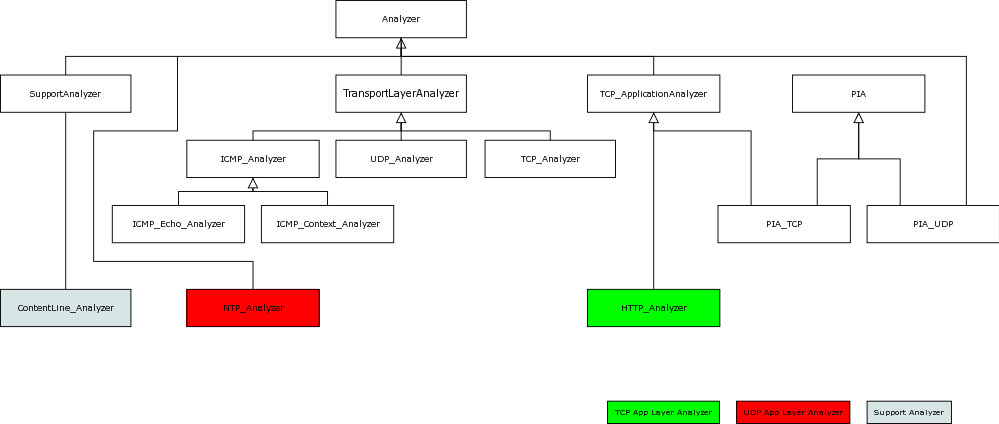
\includegraphics[width=\columnwidth]{Figures/als.png}
\caption{Class Hierarchy of Bro analyzers}
\label{als}
\end{figure}


Events can be relatively high-level (such as the establishment of a connection) or low-level (such as a TCP packet being delivered). As mentioned above, each one is represented by a list of values which provides the scripts with information to piece together what has happened. At the very least, this includes the \texttt{connection} value, which is a composite data type containing information about the stream the event happened on (for a TCP stream, this includes the source and destination addresses and ports, the state of the stream, and information about the underlying protocols). In several cases though, it is useful to provide more information for use in the script layer. When one wants to be alerted for each arriving TCP packet, for example, it is likely for a rather thorough analysis for which the \texttt{connection} value is not enough. The corresponding event, \texttt{tcp\_packet}, therefore contains much more. The following code block shows the declaration and documentation of this event: \\ \\

\textcolor{red}{review formatting once text is complete to get all the code on one page}
\begin{lstlisting}[frame=single]
## Generated for every TCP packet. This is a very low-level and expensive event
## that should be avoided when at all possible. It's usually infeasible to
## handle when processing even medium volumes of traffic in real-time.  It's
## slightly better than :bro:id:`new_packet` because it affects only TCP, but
## not much. That said, if you work from a trace and want to do some
## packet-level analysis, it may come in handy.
##
## c: The connection the packet is part of.
##
## is_orig: True if the packet was sent by the connection's originator.
##
## flags: A string with the packet's TCP flags. In the string, each character
##        corresponds to one set flag, as follows: ``S`` -> SYN; ``F`` -> FIN;
##        ``R`` -> RST; ``A`` -> ACK; ``P`` -> PUSH.
##
## seq: The packet's relative TCP sequence number.
##
## ack: If the ACK flag is set for the packet, the packet's relative ACK
##      number, else zero.
##
## len: The length of the TCP payload, as specified in the packet header.
##
## payload: The raw TCP payload. Note that this may be shorter than *len* if
##          the packet was not fully captured.
##
## .. bro:see:: new_packet packet_contents tcp_option tcp_contents tcp_rexmit
event tcp_packet%(c: connection, is_orig: bool, flags: string, seq: count, ack: count, len: count, payload: string%);
\end{lstlisting}

Each event is defined like this in a \texttt{.bif} file, which serves to define data types and functions for use in the script level. The full list of TCP events is detailed in \\ \texttt{bro/src/analyzer/protocol/tcp/event.bif}. While it is sufficient to provide the name and data types of the event's values, it is good practice to document each new event with a description of what it corresponds to, what each data field represents, and a list of the related events. \\

The MPTCP extension uses the TCP option fields (see \url{http://www.iana.org/assignments/tcp-parameters/tcp-parameters.xhtml}) for its operation. However, TCP options receive very little native support in Bro. Indeed, the only relevant event is the \texttt{tcp\_option} which provides the option kind and length. As the documentation itself states ``There is currently no way to get the actual option value, if any.''  Additionally, the function that raises this event is only executed on packets possessing a payload.\\ 

This is clearly problematic since MPTCP relies on the option value to establish the option subtype and the connection parameters such as the keys used to identify the connection, or the sequence mapping necessary to re-assemble the data from multiple subflows. MPTCP options are also crucial during the connections establishment (when no payload is given). In order to provide the "scriptland" with enough information to understand MPTCP, we must first extend the analyzer to provide new, more detailed events of what is going on in the options.

\subsection{Adding new events}
As we have seen, some work must be done at the analyzer level for MPTCP to be understood. The question remains whether to implement a new analyzer which would be a child of the TCP analyzer, or extend the TCP analyzer. The general architecture of the system is to use one analyzer per protocol. Additionally, the parsing of the TCP header is already done and it would be redundant and inefficient to do it twice. For these reasons, the choice was made to simply add the MPTCP parsing and event generation in the pre-existing analyzer. We will therefore work on \texttt{bro/src/analyzer/protocol/tcp/TCP.cc}.\\

Packets enter the analyzer through the \texttt{DeliverPacket} method. In this method we can see that the first steps are to extract the TCP header, check the flags, and update the state of the stream state. What interests us comes a little later:

\begin{lstlisting}[language = C++]
	if ( tcp_option && tcp_hdr_len > sizeof(*tp) &&
	     tcp_hdr_len <= uint32(caplen) )
		ParseTCPOptions(tp, TCPOptionEvent, this, is_orig, 0);
\end{lstlisting}

This snippet of code shows us how Bro starts the analysis of the header to detect TCP options. The first line shows what we discussed in the previous section; events are only raised when the scripts call for them. This is done thanks to the boolean \texttt{tcp\_option} being set when the script uses the event of the same name. For obvious efficiency reasons, it is not desirable to dissect the option part of the header if the end users are not interested in this behavior. If this is the case, we will call the \texttt{ParseTCPOptions} method. \\

The behavior of this function is as we would expect. It loops through each option until it reaches the end of the header, and for each valid one, it calls the \texttt{TCPOptionEvent} callback function which will populate the value list and raise the event. \\

For the simplest solution possible, it would suffice to add the value of the option to the value list and parse this in script. However, this would cause many undesired effects. Firstly, the event would be raised much more often than we would want. Secondly, this would force users to do byte-level parsing in script which the DSL is not adapted to do. Finally, scripts would be much harder to understand as they would only catch one event which would contain the whole parsing and treatment for MPTCP behavior and any other option comprehension we would want to do. \\

In order to improve this, we define ten new events and two new functions, analogous to the ones we have seen: \texttt{ParseMPTCP} and the callback function \texttt{MPTCPEvent}. Out of the ten events, eight correspond to the different subtypes that are used by the protocol. The last two are \texttt{mptcp}, a generic event indicating the use of the protocol, and \texttt{mp\_error}, indicating an option which is in some way illegal with regards to the rfc. All the events will be described in further detail in the following section. For the two functions, the first will behave exactly like \texttt{ParseTCPOptions} except for two points: it will be called if any MPTCP event is used in script, and it will only use the callback function if the option kind is 30 (MPTCP). The \texttt{MTCPEvent} is where we parse the value of the option. \\

The first step is to extract the subtype which is contained in the first four bits of the third option byte. With only this information, we can already raise the \texttt{mptcp} event if needed. If further information is required by the script, we begin a case statement on the subtype. Guards are regularly re-checked to ensure as little unneeded work as possible is done. Based on the value of the subtype, we will be able to extract the relevant fields from the header, fill the value list, and raise the correct event. If, at any point of the process, an illegal value is found (such as an option length which does not correspond to the authorized values for a given subtype), an \texttt{mp\_error} event is raised.

\subsection{Event description}
As mentioned in the previous section, ten events were added to the analyzer in order to facilitate working with the protocol, corresponding to the eight existing subtypes, a generic event, and an error event. Each one of these new events was added to \texttt{bro/src/analyzer/protocol/tcp/event.bif} along with its documentation. While the selection of which events to implement follows an intuitive choice, it is far from the only possibility. Using multiple different events allows us to minimize the in-script parsing which improves efficiency. It also allows users to focus on the behavior they want to observe. For example, when attempting to log connection information, we might not want events being fired for every DSS option detected, or care about whether an address is considered as a backup. Using more, higher-level events than what is provided in this work could also be considered. When observing the event available for standard TCP, we can see that different events exist for each step of the connection process. \\

This section will now describe the added events in detail. We will go over which elements are contained in its value list and how it is populated, as well as how it might be used to understand the protocol's behavior in script. For a reminder on the format of the MPTCP options, consult appendix \ref{mp opt format}.

\subsubsection{mptcp event}
The first implemented event is the simple \texttt{mptcp} event. This is primarily intended as a proof of concept event, but might be used to detect mptcp activity without the will to delve much deeper into details. In addition to the connection value (discussed earlier), the \texttt{mptcp} event provides the user with the option length and subtype. As such, the event can be raised early in the parsing process since we only care about extracting the subtype (it is already necessary to get the length when iterating over the different options of the header). This is all done before even beginning the main case statement that makes up most of the \texttt{MPTCPEvent} function. Once again, the practical utility of this event is limited, but it is a good starting point for the comprehension of the function thanks to its simplicity. \\

There are two important things to note with this event. First, if it will potentially be raised very often and can therefore prove impractical during real-time packet analysis (it is raised once for each MPTCP option, which means at least once per MPTCP packet). The other is that, due to how early it is raised during the option parsing, it will still be raised if an error is detected later. This makes it the only event which can be raised along with an \texttt{mp\_error} on the same option.

\subsubsection{mp\_error event}
The \texttt{mp\_error} event is one that should never arise during the use of a correct MPTCP implementation. Such errors are mainly based on the authorized lengths for the options, and either TCP or MPTCP flags. For example, a \texttt{mp\_capable} option (subtype 0) should only ever be of length 12 or 20. Furthermore, it should only be of length 20 during the final step of the three-way handshake (SYN + ACK) since it is the only time where two 64-bit keys are sent. Another example is the \texttt{DSS} option (subtype 2). In this case, the length varies not based on the TCP flags, but on the MPTCP flags contained in the option itself. \\

Given how the fields of an event's value-list are filled, it is not possible to work with incoherent values. What key should be returned if the length of a \texttt{mp\_capable} option is 10? Should we only send six bytes or assume the length is off and add two bytes from the next option or TCP payload? Given that this should not happen, we do not attempt to make the call and simply raise an error. The regular MPTCP event is not raised, and we get an \texttt{mp\_error} event instead.\\

In order to raise this event, the parsing process is carried out as normal. For each  different subtype, the length of the option is matched against the known authorized length values that the subtype can take. Further fine-tuning is done based on information from the main TCP header and the option's flags, when applicable. The values contained in the event are the same as those in the \texttt{mptcp} event, namely, the option length and subtype. Unlike the \texttt{mptcp} event however, it is raised much later in the parsing process given that the option must be analyzed in detail in order to detect the error.\\

It is worth noting that detecting a faulty implementation is far from the main aim of the software. For similar errors in the basic option parsing, incoherent length values are simply dealt with by returning -1. Given the relatively young age of the protocol, however, this event might find some use either due to new implementations containing errors or because of new attacks attempting to break the protocol.

\subsubsection{mp\_capable event}
The first of the main events, the \texttt{mp\_capable} event is raised when an MPTCP option with subtype 0 is encountered. These options are piggy-backed onto the TCP connection establishment to negotiate the use of MPTCP or lack thereof. The option value contains, in addition to the subtype, a four-bit version number of the MPTCP implementation used, eight bits of flags and one or two 64-bit keys. The option has two authorized lengths: 12 bytes for the first two steps of the three-way handshake (SYN \& SYN+ACK), or 20 bytes during the final step (ACK) which the is only time the second key is present. In order to allow the user full control over what he wants to observe, each piece of information (other than the subtype since it is always 0) is added to the event's value list. The four last bits of the third byte are passed as an integer value representing the version number, the flags are bunched together in another, and finally the eight bytes representing the keys are copied into integer values.  They are passed to the script level using Bro's own integer data type, called Count (which is 64 bits). Note that, since optional values are not supported, a second key will always be present in the event. It is therefore important to check the length in the script and to not take it into consideration should the length be 12.\\

As far as usage goes, the primary use of this event is for the detection of MPTCP connection establishment. This option tells us a lot about what is going on, both at the MPTCP level and for the TCP connection which the option belongs to. For example, a \texttt{mp\_capable} event with length 12 indicates either a TCP SYN or SYN+ACK has occurred. On further inspection, the \texttt{is\_orig} value will tell us if the packet came from the connection initiator or the responder. The first case indicates a SYN, and the second a SYN+ACK. This second packet is when the connection can generally be considered established (see the \texttt{connection\_established} event). Finally, an option with length = 20 indicates the final ACK has been sent. We could also use this information to find instances where the use of MPTCP was denied by combining new events with those of the standard TCP analyzer. Indeed, if we were to see a \texttt{mp\_capable} event on the SYN, but none after the \texttt{connection\_established} event on the same connection, this would indicate that the responder did not allow the use of the protocol and has reverted to standard TCP. \\

Other uses include the detection of unknown MPTCP versions or cryptographic choices. Furthermore, detecting and saving the keys exchanged by both hosts as well as the choice of cryptographic algorithm allows the IDS to compute the token used to identify the connection on each host, and then use this information to validate the authentication process when additional TCP connections will attempt to join the MPTCP connection. \\

Although, in the end, we still receive the whole of the information contained in the option as discussed in the first solution (passing the whole option value in \texttt{TCP\_Option} events), the advantages of this method are easy to see. We allow the script level access to the different fields of the option as variables rather than requiring byte-level parsing. We can also take the opportunity to observe how adding more events could further facilitate the comprehension of the protocol. Currently, as we have discussed in the previous paragraphs, one still has to use the same event for multiple different scenarios depending on what one wishes to observe. The \texttt{mp\_capable} event could be broken down into further, more explicit events such as a connection attempt, the establishment of the connection or its reverting to standard TCP, the first acknowledgement... in a way similar to the events that exist in the standard TCP analyzer. Doing this would also remove the use of ``placeholder'' fields such as the second key which is sent on each event, but only used in one of the three cases.

\subsubsection{mp\_join event}
\texttt{mp\_join} events correspond to options with the subtype 1. Like \texttt{mp\_capable}, they are piggy-backed onto TCP connection establishments but with one big difference: when used, the TCP connection is actually a sub-flow of the MPTCP connection it has joined. An option of the subtype contains four bits of flags and the address ID corresponding to the address the packet originated from as it is known in the MPTCP connection (independently of whether or not the actual address was modified by middle boxes along the way). The remaining fields vary depending on which step of the handshake it is on. Each one of the three steps corresponds to a set of values and a different option length which makes determining which one is taking place easy. However, filling the value list fields is made slightly harder. Based on the length, only parts of the fields are used, and the HMAC makes things worse since the actual field's length can vary. Similarly to the \texttt{mp\_capable} option, every available piece of information is sent to the script level, and it is up to the user to know which fields to use depending on the length. \\

In its use, \texttt{mp\_join} is also similar to \texttt{mp\_capable} in that it mainly serves to observe connection establishment. While it might be of some interest to simply monitor how many TCP connections are using MPTCP, we can go further and attempt to link multiple connections as being subflows of the same MPTCP connection. The token that is sent during the first SYN serves to identify which connection is being joined and should be unique on a given host. If we can observe the original key exchange for the MPTCP connection (in the MP Capable options), we can compute the tokens and match MP Joins to the corresponding connection. Of course, given that we would observe the traffic between multiple hosts, it is entirely possible to observe multiple key exchanges that would result in the same token. While unambiguous for each host, it would make matching difficult for the outside observer. \\

\subsubsection{mp\_dss event}
DSS options, subtype 2, form the main body of the connection as they are used during the actual data exchange. This option is the first we encountered which possesses many fields that are either optional or vary in length depending not on the TCP flags but on the MPTCP flags. Filling the fields of the \texttt{mp\_dss} event therefore requires parsing the five flags in order to determine which bytes correspond to which value. Like before, every individual field of the option is passed into the event. \\

This option is used to signal how the different subflows must be aggregated in order to re-assemble the data in the right order. As such, the \texttt{mp\_dss} event will primarily serve to allow observers access to the data sequence mapping to perform the same re-assembly as the hosts of the connection. However, the event can also serve to detect MPTCP connections whose establishment was not observed. Additionally, it might even be possible to determine which subflows belong to the same connection if links between the sequence mappings can be established. Finally, the DSS option is also responsible for signalling when a host has no more data to send on this connection.\\

An important note regarding this event is that DSS options are carried on every MPTCP packet after the connection establishment, making it a very common option when the protocol is in use. As such, the event will be raised fairly often, which may cause performance issues.

\subsubsection{mp\_add\_addr event}
The \texttt{mp\_add\_addr} event is raised when an MPTCP option of subtype 3 is seen. These options are part of the address signalling mechanism of MPTCP. Though rather straightforward, some field values once again depend on the information contained within the same option. The option contains the IP version of the address being added and the address ID that will be used to identify it within the MPTCP connection. These two values can be simply put into the value list as integers. The next important field is the address itself. Using the IP version lets us know how long (32 or 128 bits) the address is. In order to pass it to the script, we use Bro's built-in \texttt{addr} data type. This is a high-level structure which is able to handle both IPv4 and IPv6 addresses and even host names. The last piece of information is the port number. This field is one of the two optional fields whose presence is not indicated by either the TCP or MPTCP flags. The only way to detect its presence during the parsing is whether the option length is a multiple of four (in which case it is absent), or not (in which case it is present). Though simply given as an integer, Bro also has a  \texttt{port} data structure which can indicate the protocol associated with the given port. \\

In order to observe connection establishment, the \texttt{mp\_add\_addr} can help reduce ambiguity with joins. As we mentioned earlier, the tokens used to identify connections are supposed to be unique for a given host, but are not expected to be so across multiple hosts. Memorizing the addresses that are advertised over a given MPTCP connection as well as its token can help reduce the chance of colliding tokens. Indeed, if two MPTCP connections A and B use the same token, and an address is advertised over connection A, a join coming from that address can probably be assumed to belong to connection A and not B. \\

Additionally, we can even match subflows to their MPTCP connection based solely on the addresses advertised and used during joins, which allows us to monitor connections without re-computing the cryptographic functions, or if the key exchange was not observed. However, this method cannot account for the modification of addresses by middleboxes, and we risk collisions again if two hosts advertise the same address.

\subsubsection{mp\_remove\_addr event}
With subtype 4, REMOVE ADDR options are the opposite of ADD ADDR. It is also one of the simplest options of the protocol; since each address that was advertised over the MPTCP connection is uniquely identified by an ID, that ID is sufficient to unambiguously remove it from the available addresses. However, it does have a small subtlety which is that a single REMOVE ADDR option can remove an arbitrary (within the limits of the TCP option space) number of addresses. The number is deduced from the option length, one byte being used per address ID. Rather than letting the script determine how many addresses are affected by a single \texttt{mp\_remove\_addr} event, one event is raised for each address, each one containing one ID. \\

The \texttt{mp\_remove\_addr} can be used to optimize memory use by allowing us to remove addresses from memory as soon as the MPTCP connection stops using them. Some use might also be found in trying to understand how a given host decides which addresses to make available and when.

\subsubsection{mp\_prio event}
The \texttt{mp\_prio} event contains the other optional field not indicated by anything other than option length. It is a very straightforward option that simply changes the status of a subflow to backup or back to regular. Its use is rather limited, but one may be interested in observing which links hosts prioritize.

\subsubsection{mp\_fastclose \& mp\_fail events}
The last two events, corresponding to subtypes 6 and 7 respectively, are both relatively simple to generate, having few and fixed fields. The data is simply passed to the scripts as integers. In both cases, their use deals with the termination of MPTCP on the connection. \texttt{mp\_fastclose}, being used for abrupt termination of an MPTCP connection, can primarily be used for resource management (removing connection state from memory when it closes). \texttt{mp\_fail} has more interesting applications since it can potentially reveal the existence of middleboxes that deny the use of MPTCP between two hosts that are otherwise willing to use the protocol.


\section{Script-level Functionalities}


\section{Testing}


\section{Further Considerations}


\section{Conclusion}



%\mainmatter % Begin numeric (1,2,3...) page numbering

\pagestyle{fancy} % Return the page headers back to the "fancy" style

% Include the chapters of the thesis as separate files from the Chapters folder
% Uncomment the lines as you write the chapters
\pagebreak
%\input{./Chapters/introduction.tex}
%\input{./Chapters/high_level_view_of_the_website.tex}
%\pagebreak
%\input{./Chapters/functional_requirements.tex}
%\pagebreak
%\input{./Chapters/non_functional_requirements.tex}
%\pagebreak
%\input{./Chapters/clarification_questions_and_suggestions.tex}
%\pagebreak
%\input{./Chapters/selected_extensions.tex}
%


\chapter{Conclusion} \label{chap:conclusion}
This concludes our work on Deep Packet Inspection with Multipath TCP. As we have seen, the development and deployment is not limited to conceptualizing it and implementing. For a protocol to achieve large scale success on today's internet, compliance with commonly used networking tools is just as important as good design. In addition to the common challenges of creating a new protocol, our overview of MPTCP has shown that this protocol in particular brings about new challenges that break many common assumptions on modern networks.\\

In an effort to improve existing tools to work with MPTCP, we have present the Bro IDS, a powerful and flexible tool to network analysis and intrusion detection. By explaining how the system functions, we exposed which parts needed to be worked on in order to allow Bro to understand and produce meaningful results with MPTCP. We discussed the two main components of Bro: the Event Engine which parses packets to raise events has been modified in order to transfer the binary MPTCP information contained in the TCP options to the powerful Policy Script Interpreter, and to do so in an easily understandable manner. With the new events being raised, we have been able to produce scripts which can exploit the information in order to showcase important behavior within the protocol. \\

While presenting the scripts, we outlined potential attacks that may be used in the future against the protocol. Doing so brings us back to original premise of the thesis; adapting network monitoring and security tools is essential to ensure that we will be able to detect and counteract future attacks. Off course, we have seen that there is still much that can be done. As the protocol matures and more and more people use it and work on it, it is most likely that new techniques for intrusion detection tailored to MPTCP will emerge. In the end, we must bare mind one thing; if MPTCP changes the way we send data, it will also make us change the way we observe these transfers.
%\chapter{Introduction} \label{chap:intro}
Creating a new protocol and ensuring its large scale deployment and use over the internet presents a series of wide ranging challenges. Multipath TCP (MPTCP) has taken many of these considerations into account from the start of its development, namely going to great lengths to ensure retro-compatibility with regular TCP, mechanisms for working over NATs and certain other middle boxes, and fall-back signaling to revert to TCP if needed. Thanks to this, it has met a level of success which is rare for a protocol of its type. However, there are still many challenges ahead to ensure that the protocol can reach a level of usage comparable to that of regular TCP. \\

One such challenge is security. While securing the protocol itself through the use of randomized  sequence numbers, cryptography, and careful design is important, many attacks use legitimate protocol operations and can only be detected as attacks when looking at the bigger picture. Even when a protocol has been designed to cope or to mitigate a problem, a network operator may still wish to be alerted when such an attack is taking place. Lets take TCP as an example. If a server receives a SYN packet, replies with a SYN+ACK, and no final ACK arrives, the connection is in a partially opened state until it times out. This is regular operation and is certainly not a problem from the protocol's point of view. The issue arises when thousands of SYN packets arrive within a short window, a SYN flooding attack. None of the individual connections is odd, but a security system observing the traffic and capable of understanding TCP will easily identify this as an attack. Even with ways to deal with this problem, such as stateless server operation during the connection establishment, the network's operators would likely want to be informed that this attack is happening/has happened. \\

This is just one example to illustrate the need for security and monitoring tools that understand the protocols in use within the network. Many efforts have already been made in in order to adapt commonly used tools to MPTCP. For example, Wireshark \cite{wireshark} was patched in order to display MPTCP options and their field values \cite{mpwireshark}, as we can  see in figure \ref{pic:wshark demo}. However, it does not yet provide the function to ``follow'' an MPTCP stream as it can a regular TCP stream. The TCPdump \cite{tcpdump} command line utility was also updated in order to display MPTCP information \cite{mptcpdump}. Both the Wireshark and TCP dump extensions are now featured in the standard distribution of these programs. The packet manipulation program Scapy \cite{scapy} was also given an MPTCP update, allowing it to read, display, modify and write MPTCP options \cite{mpscapy} .   \\

\begin{figure}[!t]
\centering
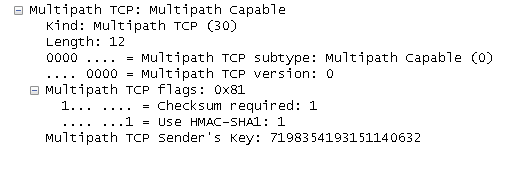
\includegraphics[width=\columnwidth]{Figures/wiresharkdemo.png}
\caption{MPTCP option as seen in Wireshark}
\label{pic:wshark demo}
\end{figure}

This work is intended as a continuation of those efforts in order to bring a new security tool up to speed with MPTCP: Deep Packet Inspection (DPI). DPI is a method generally employed within intrusion detection systems (IDS). While a lot of packet analysis usually stops at headers, DPI can provide byte-level inspection of the whole packet, including the payload. While many systems use DPI, we have chosen to work with the Bro network analysis framework \cite{bro} . Bro is a powerful and flexible system which also also has the great advantages of being widely used and open source. As part of our work, we have extend Bro to provide MPTCP comprehension, and built scripts to use these new functionalities for MPTCP analysis. Until now, whenever Bro encountered a packet using MPTCP, it would be treated as a regular TCP packet. Thus, though the operation of the system was not jeopardized, users were incapable of of retrieving MPTCP related information. Furthermore, the subsequent analysis of application-layer protocols became impossible if the MPTCP stream was split over multiple connections, since Bro is incapable of reassembling subflows into a single data stream. \\

In this document, we will begin with two chapters presenting the inner workings of the Multipath TCP protocol in chapter \ref{chap:mptcp} and the Bro framework in chapter \ref{chap:bro}. We will then describe the modifications that have been made within Bro in order to make the system MPTCP compliant in chapter \ref{chap:events} . In chapter \ref{chap:script} , we will describe how the modified system can be used to extract meaningful information from analyzed traffic and packet traces. With the main development explained, chapter \ref{chap:test} will then describe how both the Bro modifications and scripts were tested. Finally, we will discuss further work which can be done on the subject in chapter \ref{chap:further} .
%\input{./Chapters/ContexteGlobal.tex}
%\input{./Chapters/Localite.tex}
%\input{./Chapters/abreprob.tex}
%\input{./Chapters/Etatdelart.tex}
%\input{./Chapters/Recommandations.tex}
%\input{./Chapters/ccl.tex}




%----------------------------------------------------------------------------------------
%	BIBLIOGRAPHY
%----------------------------------------------------------------------------------------
%\newpage
%\section{Bibliography}
%\label{Bibliography}
%
%\lhead{\vspace{1em}\emph{Bibliography}} % Change the page header to say "Bibliography"
%
%\bibliographystyle{unsrtnat} % Use the "unsrtnat" BibTeX style for formatting the Bibliography
%
%\bibliography{Bibliography} % The references (bibliography) information are stored in the file named "Bibliography.bib"

%----------------------------------------------------------------------------------------
%	THESIS CONTENT - APPENDICES
%----------------------------------------------------------------------------------------

\addtocontents{toc}{\vspace{2em}} % Add a gap in the Contents, for aesthetics
%
\appendix % Cue to tell LaTeX that the following 'chapters' are Appendices
\section{MPTCP Option Formats} \label{mp opt format}

              

%
%% Include the appendices of the thesis as separate files from the Appendices folder
%% Uncomment the lines as you write the Appendices
%
%\input{./Appendices/resultats}
%\input{./Appendices/finances}
%\input{./Appendices/methodo}
%
%\addtocontents{toc}{\vspace{2em}} % Add a gap in the Contents, for aesthetics
%
%%\backmatter


\end{document}  